%----------------------------------------------------------------------------------------
%       PACKAGES AND OTHER DOCUMENT CONFIGURATIONS
%----------------------------------------------------------------------------------------

\documentclass{article}

\usepackage{fancyhdr} % Required for custom headers
\usepackage{lastpage} % Required to determine the last page for the footer
\usepackage{extramarks} % Required for headers and footers
\usepackage[usenames,dvipsnames]{color} % Required for custom colors
\usepackage{graphicx} % Required to insert images
\usepackage{listings} % Required for insertion of code
\usepackage{grace}
\usepackage{courier} % Required for the courier font
\usepackage{lipsum} % Used for inserting dummy 'Lorem ipsum' text into the template

% Margins
\topmargin=-0.45in
\evensidemargin=0in
\oddsidemargin=0in
\textwidth=6.5in
\textheight=9.0in
\headsep=0.25in

\linespread{1.1} % Line spacing

% Set up the header and footer
\pagestyle{fancy}
\lhead{\gphixAuthorName} % Top left header
\chead{\gphixCHead} % Top center head
\rhead{\firstxmark} % Top right header
\lfoot{\lastxmark} % Bottom left footer
\cfoot{} % Bottom center footer
\rfoot{Page\ \thepage\ of\ \protect\pageref{LastPage}} % Bottom right footer
\renewcommand\headrulewidth{0.4pt} % Size of the header rule
\renewcommand\footrulewidth{0.4pt} % Size of the footer rule

\setlength\parindent{0pt} % Removes all indentation from paragraphs



% --------------------------------------------------------------------------------------
%       SET UP GRACE SCRIPT LISTINGS
% --------------------------------------------------------------------------------------

\newcommand{\gracescript}[2] {

    \begin{itemize}
    \item[]\lstinputlisting[caption=#2,label=#1]{#1.grace}
    \end{itemize}

}



%----------------------------------------------------------------------------------------
%       USER DEFINED COMMANDS
%----------------------------------------------------------------------------------------

\newcommand{\gphixTitle}{Grace - Phix} % Assignment title
\newcommand{\gphixCHead}{Grace - Phix : API} % Center Header
\newcommand{\gphixAuthorName}{Alex Sandilands} % Author Name
\newcommand{\gphixCurDate}{Friday,\ January\ 24,\ 2014} % Current Date

%----------------------------------------------------------------------------------------
%       TITLE PAGE
%----------------------------------------------------------------------------------------

\title {
    \vspace{2in}
    \textmd{\textbf{\gphixTitle}}\\
    \normalsize\vspace{0.1in}\small{Graphics API for the Grace programming lanuage}\\
    \vspace{0.1in}\large{\textit{Last updated on:\\}}
    \vspace{0.1in}\textbf{21-01-2014}
    \vspace{3in}
}

\author{\textbf{\gphixAuthorName}}
\date{} % Leave empty to stop date from appearing


%----------------------------------------------------------------------------------------
%       DOCUMENT STRUCTURE
%----------------------------------------------------------------------------------------

% Header and footer for when a page split occurs within a module environments
\newcommand{\enterModuleHeader}[1] {

    \nobreak\extramarks{#1}{#1 continued on next page\ldots}\nobreak
    \nobreak\extramarks{#1 (continued)}{#1 continued on next page\ldots}\nobreak

}

% Header and footer for when a page split occurs between module environments
\newcommand{\exitModuleHeader}[1]{

    \nobreak\extramarks{#1 (continued)}{#1 continued on next page\ldots}\nobreak
    \nobreak\extramarks{#1}{}\nobreak

}

\newcommand{\moduleName}{}
\newenvironment{module}[1] {

    \renewcommand{\moduleName}{#1}
    \section{\moduleName}

    % Header and footer within the environment
    \enterModuleHeader{\moduleName}

}{
    % Header and footer after the environment
    \exitModuleHeader{\moduleName}
}


\newcommand{\moduleSectionName}{}
\newenvironment{moduleSection}[1] {

    \renewcommand{\moduleSectionName}{#1}

    \subsection{\moduleSectionName}

    % Header and footer within the environment
    \enterModuleHeader{\moduleName}

}{
    % Header and footer after the environment
    \exitModuleHeader{\moduleName}
}


\begin{document}

\grace

\maketitle

%----------------------------------------------------------------------------------------
%       TABLE OF CONTENTS
%----------------------------------------------------------------------------------------

%\setcounter{tocdepth}{1} % Uncomment this line to stop subsections being listed in the ToC

\newpage
\tableofcontents
\newpage


%----------------------------------------------------------------------------------------
%       GRAPHICS MODULE
%----------------------------------------------------------------------------------------

\section{Summary}

This is a very simple graphics api, designed to be flexible with many different backends.
Currently, the GTK+3 backend is nearing completion. Animations are going to be added very soon
then it will be finished.\\

We are also currently working on a Javascript backend, so the graphics library can be run on
the web IDE as well. The idea is that if someone wrote a program using the GTK backend library,
their code could also work on the web IDE without changing anything.\\

The library has been designed so the backend can be very easily changed, so if other graphics
sources are ported into Grace they can be used with Grace-Phix.\\


\subsection{Component Hierarchy}
This is a very basic draft of the hierarchy of how the graphical components work.
A nicer diagram will be made soon.

\vspace{0.5in}

\begin{center}
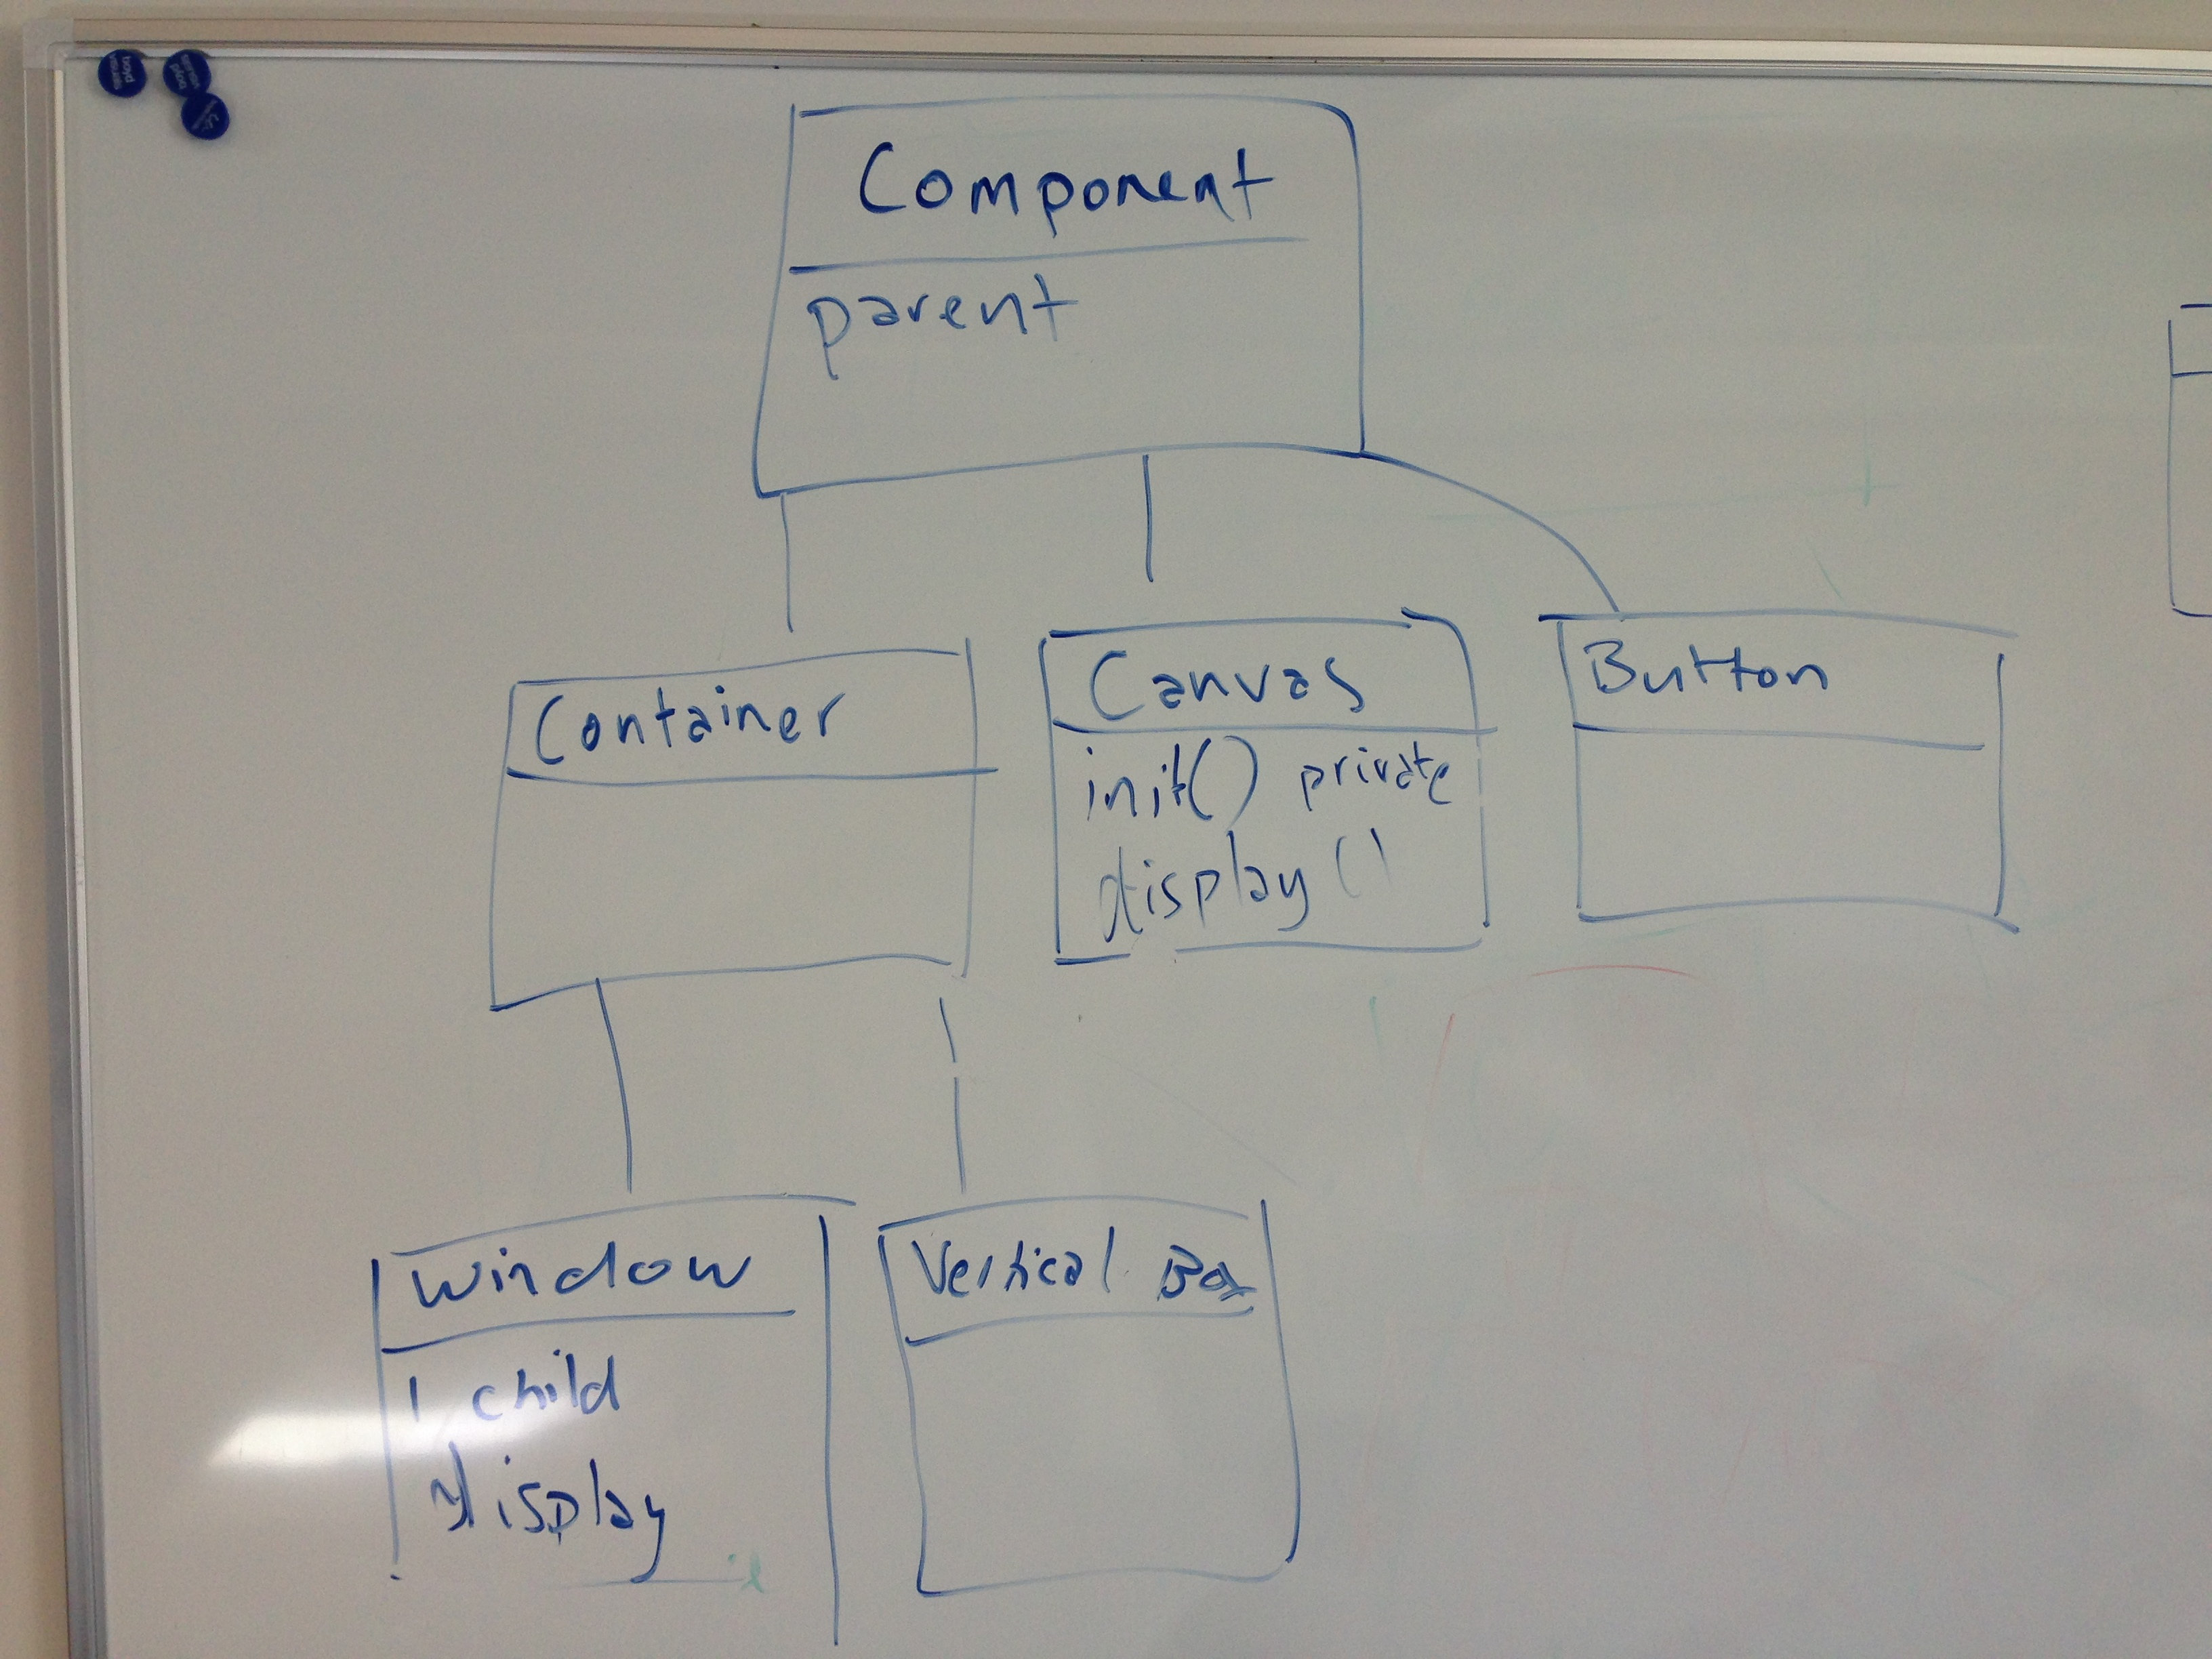
\includegraphics[width=0.75\columnwidth]{images/hierarchy_diagram_draft}
\end{center}


\clearpage

\begin{module}{Graphics}

This module is a list of object constructors for all of the graphical components
this library uses. It also has constructors for the drawable shapes, which can be
used and combined to create new drawable objects that can be added and drawn on
a canvas. It is split up into sections for readability, based on which type of
objects the methods are creating.\\
This is the main module that will be imported into a program when using the graphics
library

\begin{moduleSection}{Interface}

Listing \ref{code/graphics_interface} shows the interface for Grace-Phix graphics.
\gracescript{code/graphics_interface}{Grace-Phix graphics interface}

\end{moduleSection}

\clearpage

\end{module}



\begin{module}{Window}

This component is a top level graphical frame, which is required
for anything that needs to be displayed. It is also of type container
as it can contain other components which get displayed in the window.
Whenever you add a new component to the window it gets displayed at the
bottom, as the window uses a vertical box. You can add other boxes
to the window if you want components to be displayed in different directions
and orders.

\begin{moduleSection}{Interface}

Listing \ref{code/window_interface} shows the interface for a Grace-Phix window.
\gracescript{code/window_interface}{Grace-Phix window interface}

\end{moduleSection}

\clearpage

\end{module}



\begin{module}{Canvas}

This component is a display buffer. It contains a list of drawable objects
which get painted to the buffer and can be manipulated.
Dispite appearing to have similar methods as a container, it is not as it
doesn't contain components, only drawables.
The canvas can have external drawables objects added to it, or it can create
it's own basic drawables directly.

\begin{moduleSection}{Interface}

Listing \ref{code/canvas_interface} shows the interface for a Grace-Phix canvas.
\gracescript{code/canvas_interface}{Grace-Phix canvas interface}

\end{moduleSection}

\clearpage

\end{module}



\begin{module}{Drawable}

This module contains all of the basic objects that can be painted on a canvas.
The canvas can paint any object that is of type Drawable. You can create
your own object that is made up of lots of these basic drawable types, make sure
it is of type Drawable, then simply add it to the canvas to be drawn.

\begin{moduleSection}{Interface}

Listing \ref{code/drawable_interface} shows the interface for a Grace-Phix drawable.
\gracescript{code/drawable_interface}{Grace-Phix drawable interface}

\end{moduleSection}

\clearpage

\end{module}



\begin{module}{Components}

This module has the graphical components that are displayed on the screen.
Other than utility objetcs and drawables, all objects in Grace-Phix are components at
the top level. For example, a verticale box is a component and a container, so it can contain other components, including other containers.
Only minor components are defined in this module, the large ones such as window and canvas
have their own modules.

\begin{moduleSection}{Interface}

Listing \ref{code/components_interface} shows the interface for Grace-Phix components.
\gracescript{code/components_interface}{Grace-Phix components interface}

\end{moduleSection}

\clearpage

\end{module}


\end{document}